%& --shell-escape

\documentclass[13pt]{beamer}
\usetheme{CambridgeUS}
\usecolortheme{dolphin}

\usepackage{microtype}
\usepackage{amsmath}
\usepackage{lmodern}
\usepackage{tikz}
\usepackage[czech,slovak]{babel}
\usepackage[utf8x]{inputenc}
\usepackage{times}
\usepackage{pgfpages}
\usepackage{amssymb}
\usepackage{graphicx}
\usepackage{listings}
\usepackage{minted}
\usepackage[showboxes, overlay]{textpos}

\setbeameroption{show notes on second screen=right} % Both
\setbeamertemplate{show notes}{\pagecolor{yellow!5}\insertnote}\usepackage{palatino}

\usetikzlibrary{calc,trees,positioning,arrows,chains,shapes.geometric,%
    decorations.pathreplacing,decorations.pathmorphing,shapes,%
    matrix,shapes.symbols}

\title{Interpret jazyka IFJ16 (a/4/I)}
\subtitle{Semestrální projekt IFJ}
\institute{FIT VUT Brno}
\author[ Tamaškovič,Vaško,Vaško,Záleský,Zárybnický]
{Marek~Tamaškovič, Martin~Vaško, Michal~Vaško, Jiří~Záleský, Jakub~Zárybnický}
\date{14. prosince 2016}

\newsavebox{\grammarbox}

\begin{document}

\begin{frame}
  \titlepage
  \note[item]{Varianta a/4/I - Knuth–Morris–Pratt algoritmus pre vyhledáni podřetezce v řetezci, jako seřaďovací algoritmus byl použit List-Merge a tabulka symbolu byla implementovaná pomoci BVS.}
\end{frame}

\section{Úvod}

\subsection{Zadání}

\section{Architektura}

\begin{frame}{Přehled architektury}
  \begin{center}
\begin{tikzpicture}
[box/.style={rectangle, rounded corners, draw=black,
minimum width=5em, minimum height=2em}]
\node[box] (local1) at (7,-2) {Local SymTable};
\node[box] (local2) at (7,-3.5) {Local SymTable};
\node[box] (interpret) at (3.5,-3.5) {interpret.c};
\node[box] (sanity) at (3.5,-2) {sanity.c};
\node[box] (parser) at (3.5,0) {parser.c};
\node[box] (lexer) at (3.5,1.5) {lexer.c};
\node (file) at (-1.5,1.5) {FILE *};
\node[box] (global) at (-1.5,-3.5) {Global SymTable};
\node[box] (ifj) at (-1.5,0) {ifj16.c};
\node (stdin) at (2.75,-4.5) {stdin};
\node (stdout) at (4.25,-4.5) {stdout};

 \begin{scope}[every node/.style={scale=.7}]
\path[-latex] (ifj) edge node[right]{fopen} (file)
				 edge node[above]{parseFile} (parser)
				 edge node[above,rotate=-21]{runSemanticAnalysis} (sanity)
				 edge node[above,rotate=-35]{evalMain} (interpret);
\draw[-latex]  (file) edge node[above]{getChar} (lexer);
\draw[-latex]  (parser) [bend right=10]edge node[right]{getNextToken} (lexer);
\draw[-latex]  (lexer) [bend right=10]edge node[left]{Token*} (parser);
\draw[-latex]  (parser) edge (global);
\draw[-latex]  (global) edge (sanity);
\draw[-latex]  (sanity) [bend right=10]edge (local1);
\draw[-latex]  (local1) [bend right=10]edge (sanity);
\draw[-latex]  (interpret) [bend right=10]edge (local2);
\draw[-latex]  (local2) [bend right=10]edge (interpret);
\draw[-latex]  (interpret) edge (stdout);
\draw[-latex]  (stdin) edge (interpret);
\draw[-latex]  (global) [bend right=10]edge (interpret);
\draw[-latex]  (interpret) [bend right=10]edge (global);
\end{scope}
\end{tikzpicture}
  \end{center}
\end{frame}

\begin{frame}[fragile]{Datové typy (AST)}

\textblockcolour{white}
\TPMargin{5pt}

\begin{textblock}{10}(0, -4.5)
\begin{minted}{haskell}
data Value = ValInteger Int
           | ValDouble Double
           | ValBool Bool
           | ValString String
\end{minted}
\end{textblock}

\pause
\begin{textblock}{16}(0, 0)
\begin{minted}{haskell}
data UnaryOp = PreInc | PostInc | PreDec | ...
data BinaryOp = Equal | NotEqual | Less | ...
data Expression = ExprFuncall String [Expression]
                | ExprValue Value
                | ExprReference String
                | ExprUnary UnaryOp Expression
                | ExprBinary BinaryOp Expression Expression
\end{minted}
\end{textblock}

\pause
\begin{textblock}{14}(2, -3.5)
\begin{minted}{haskell}
data Type = TString | TInteger | TDouble | ...
data Declaration = Declaration Type String
data Command = CmdDeclare Declaration
             | CmdDefine Declaration Expression
             | CmdAssign String Expression
             | CmdBlock [Command]
             | CmdReturn (Maybe Expression)
             | CmdFor { var :: Declaration
             	 , init :: Expression
                      , cond :: Expression
                      , iter :: Expression
                      , block :: Command }
             | ...
\end{minted}
\end{textblock}

\pause
\begin{textblock}{13.5}(1.5, 2)
\begin{minted}{haskell}
data Function = { fnName :: String
                , fnReturnType :: Type
                , fnArguments :: [Declaration]
                , fnBody :: [Command]
                , fnBuiltin :: Bool
                }
\end{minted}
\end{textblock}

\end{frame}

\begin{frame}{Hierarchie typů}
\end{frame}

\section{Komponenty}
\subsection{Lexikální analýza}

\begin{frame}{Lexikální analýza}
  \begin{itemize}
    \item makro GET\_CHAR (implicitní zpracování chyb)
    \item token ví, na jakém řádku a sloupci se nachází
    \item UNARY, BOOLOP, CYCLES, BASE
    \item mírně problémy s rozšířením BASE (převod desetinných čísel)
 \end{itemize}
  \note[item]{Lexikálna analýza funguje na princípe konečného automatu. Ten načíta zo vstupného súboru znaky, lexikálna analýza ich vyhodnotí a posiela ako tokeny do syntaktického analyzátora. Tokeny obsahujú informácie o type a obsahu. Taktiež sme si ale implementovali aj macro GetChar vďaka ktorému dokáže náš token posielať nielen základne informácie o type ci obsahu ale pridáva k nim aj ďalšie informácie o riadku a stĺpci na ktorej sa tieto znaky v interpretovanom súbore nachádzajú a výrazne tak uľahčuje prácu syntaktickému analyzátoru.}
  \note[item] {Ako si môžete všimnúť aj v diagrame ,implementovali sme aj všetky dostupne rozšírenia. Menovite BOOLOP , Unarne ale aj cykly typu for a do-while. Menší problém však bol s rozšírením BASE. Konkrétne s prevodom hexadecimálnej sústavy v desatinnom tvare. Tu sme museli implementovať funkciu hexToDbl ktorá to následne prekonvertovala do desiatkovej sústavy.}
\end{frame}

\begin{frame}{Stavový diagram lexeru}
  \begin{center}
    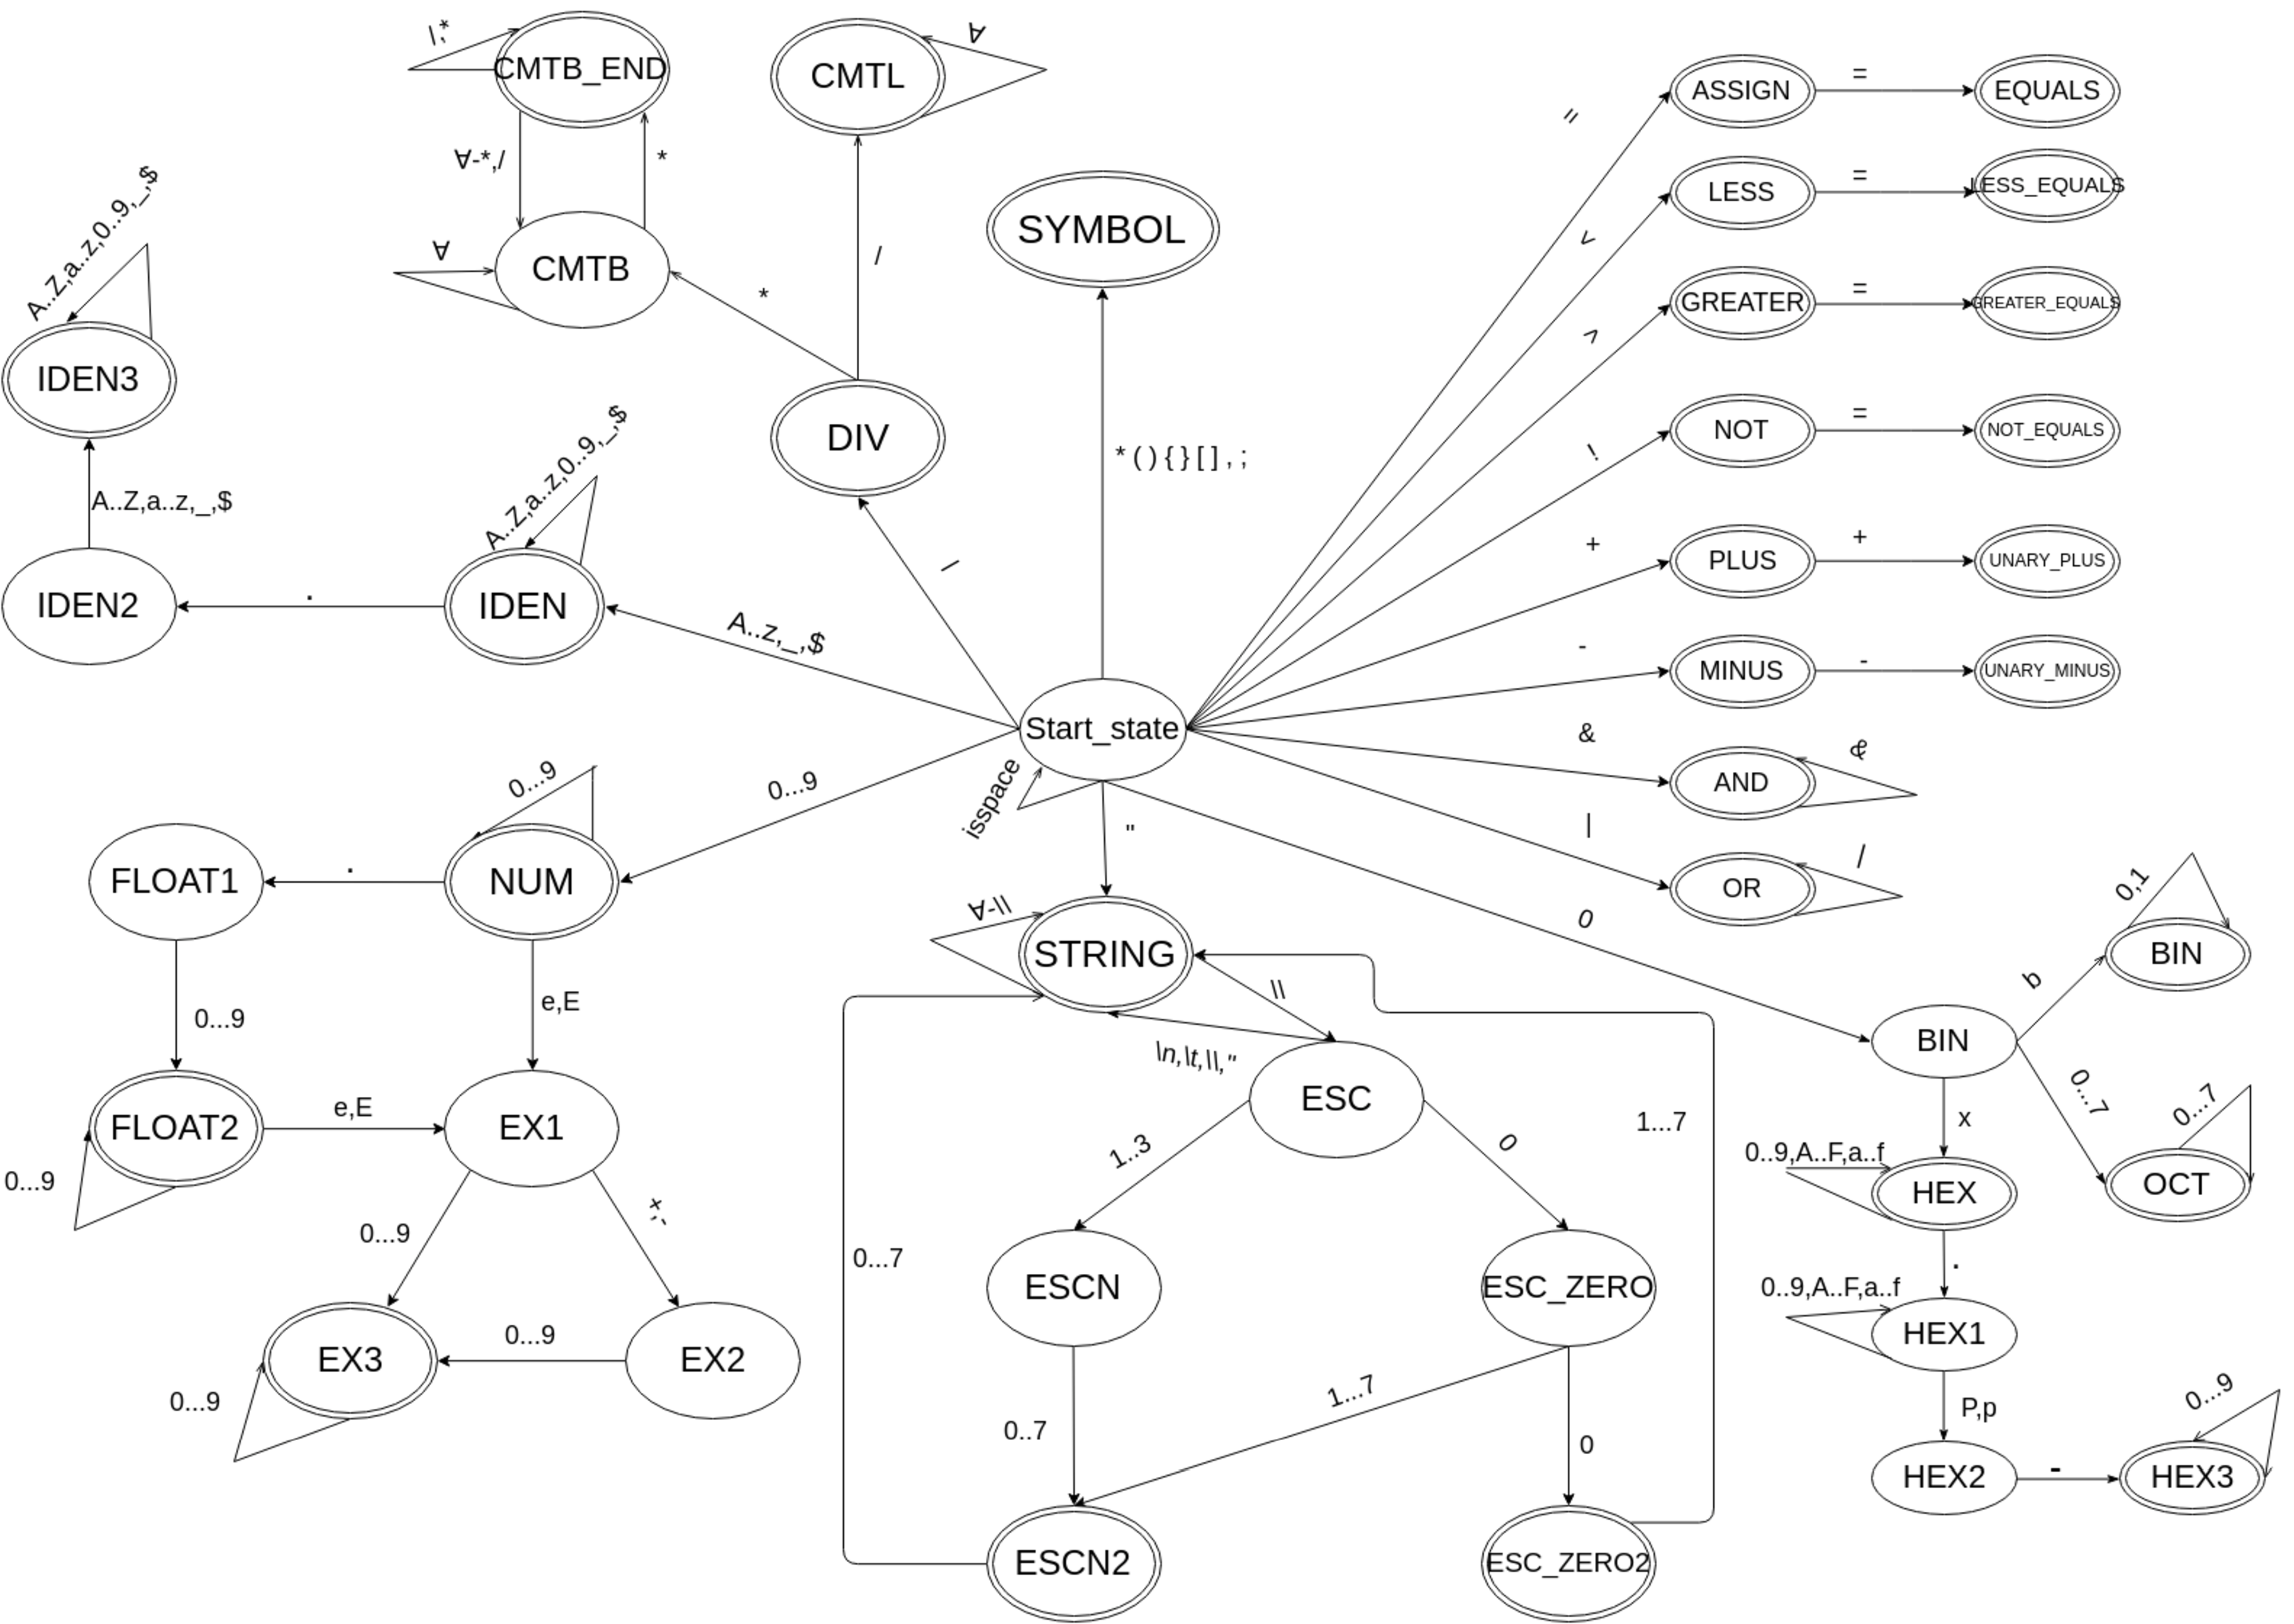
\includegraphics[width=0.8\textwidth]{img/lex1.pdf}
  \end{center}
\note[item]{ Čo sa týka diagram ktorý vidíte na obrazovke, urobil som par zmien aby sa zvýšila prehľadnosť diagramu. Konkrétne pri Symboloch kde som vytvoril jeden stav a pomenoval ho symbol a tam poslal všetky symboly ktoré nepotrebovali implementovať stav v automate a taktiež pri ďalších symboloch ako >,<,+++,-- atď.(o ktoré symboly sa jedna je  vidno na diagrame, pravá strana) kde som miesto jedného stavu pridal aj druhy ktorý v kóde nie je a to preto aby som názorne ukázal ako prebieha jednotlivé načítanie znakov v lexikálnej analýze i aj keď nie sú už súčasnou stavov avšak úplne zodpovedajú tomu ako lexikálna analýza funguje.}
\end{frame}

\subsection{Syntaktická analýza}

\begin{frame}{Syntaktická analýza}
  \begin{itemize}
  \item analýza rekurzivním sestupem, precedenční analýza
  \item stávající implementace je druhá, původní byla rekurzivním sestupem všude
  \item nová implementace mnohem delší a méně elegantní, i když asi rychlejší
  \item bez použití maker by bylo kódu cca o 300\% víc
  \item např. \texttt{expectSymbol(l, SYM\_SEMI);} odpovídá 15 řádkům kódu
  \item umožňuje skoro přímý přepis gramatiky do C
  \item UNARY - podmíněné nahrazení \textbf{-} za \textbf{u-} (za znaky \$, ( a za operátory)
  \end{itemize}
\note[item]{Hlavní část syn.al. je rekurzivním sestupem, tj. jednotlivé funkce reprezentují produkce gramatiky (parseFunction apod.).}
\note[item]{Výrazy jsou dle zadání precedenční analýzou - původně, kvůli nepochopení zadání jsme dělali vše rekurzivním sestupem (tam taky analyzujeme precedenci, ne?)}
\note[item]{Většina kódu této částu je z maker, které umožňují skoro 1:1 přepsat gramatiku do kódu - bez nich by taky kód čtyřikrát delší.}
\note[item]{UNARY - jediný problém, co tam byl (kromě neelegance a délky kódu), bylo unární mínus, které se nakonec z klasického binárního nahrazuje ``ručně'', podle předcházejícího znaku.}
\note[item]{Gramatika a tabulka pro referenci na dalších slidech}
\end{frame}

\begin{frame}[fragile]{LL gramatika}
\begin{lrbox}{\grammarbox}%
    \begin{lstlisting}%
ifj16 = \$ | class ifj16
class = "class" "{" classBody
classBody = "}" | "static" type simpleId classBody'
classBody' = ";"
           | "=" expression ";"
           | "(" declarationList "{" functionBody
functionBody = "}"
              | type simpleId(q) functionBody'
              | command
functionBody' = ";" | "=" expression ";"
command = "if" "(" expression ")" command
        | "while" "(" expression ")" command
        | "do" command "while" "(" expression ")" ";"
        | "for" "(" type simpleId for'
        | "return" return'
        | "{" commandList
        | "break" ";"
        | "continue" ";"
        | anyId command'
for' = ";" for'' | "=" expression ";" for''
for'' = expression ";" anyId "=" expression ")" command
return' = ";" | expression ";"
commandList = "}" | command commandList
command' = "(" argumentList ";" | "=" expression ";"
declarationList  = ")" | type simpleId declarationList'
declarationList' = ")" | "," type simpleId declarationList'
argumentList  = ")" | expression argumentList'
argumentList' = ")" | "," expression argumentList'
type = "int" | "double" | "boolean" | "String" | "void"
anyId = simpleId | compoundId
    \end{lstlisting}%
\end{lrbox}%
\scalebox{0.52}{\usebox{\grammarbox}}
\end{frame}

\begin{frame}{Precedenční tabulka}
\scalebox{0.55}{
\begin{tabular}[pos]{r|l|l|l|l|l|l|l|l|l|l|l|l|l|l|l|l|l|l|l|l|l|l|l}
    &(&)&++&--&u-& !& *& /& +& -& <& >&<=&>=&==&!=&\&\&&$\|$&id&li&tf&,& \$ \\
    (& L& E& L& L& L& L& L& L& L& L& L& L& L& L& L& L& L& L& L& L& L& E& O \\
    )& O& G& O& O& O& O& G& G& G& G& G& G& G& G& G& G& G& G& O& O& O& G& G \\
    ++& O& G& G& G& O& O& G& G& G& G& G& G& G& G& G& G& G& G& L& O& O& G& G \\
    --& O& G& G& G& O& O& G& G& G& G& G& G& G& G& G& G& G& G& L& O& O& G& G \\
    u-& L& G& O& O& G& G& G& G& G& G& G& G& G& G& G& G& G& G& L& G& L& O& G \\
    !& L& G& O& O& G& G& G& G& G& G& G& G& G& G& G& G& G& G& L& G& L& O& G \\
    *& L& G& L& L& L& L& G& G& G& G& G& G& G& G& G& G& G& G& L& L& L& G& G \\
    /& L& G& L& L& L& L& G& G& G& G& G& G& G& G& G& G& G& G& L& L& L& G& G \\
    +& L& G& L& L& L& L& L& L& G& G& G& G& G& G& G& G& G& G& L& L& L& G& G \\
    -& L& G& L& L& L& L& L& L& G& G& G& G& G& G& G& G& G& G& L& L& L& G& G \\
    <& L& G& L& L& L& L& L& L& L& L& G& G& G& G& G& G& G& G& L& L& L& G& G \\
    >& L& G& L& L& L& L& L& L& L& L& G& G& G& G& G& G& G& G& L& L& L& G& G \\
    <=& L& G& L& L& L& L& L& L& L& L& G& G& G& G& G& G& G& G& L& L& L& G& G \\
    >=& L& G& L& L& L& L& L& L& L& L& G& G& G& G& G& G& G& G& L& L& L& G& G \\
    ==& L& G& L& L& L& L& L& L& L& L& L& L& L& L& G& G& G& G& L& L& L& G& G \\
    !=& L& G& L& L& L& L& L& L& L& L& L& L& L& L& G& G& G& G& L& L& L& G& G \\
    \&\&& L& G& L& L& L& L& L& L& L& L& L& L& L& L& L& L& G& G& L& L& L& G& G \\
    $\|$& L& G& L& L& L& L& L& L& L& L& L& L& L& L& L& L& L& G& L& L& L& G& G \\
    id& E& G& G& G& O& O& G& G& G& G& G& G& G& G& G& G& G& G& O& O& O& G& G \\
    literal& O& G& O& O& O& O& G& G& G& G& G& G& G& G& G& G& G& G& O& O& O& G& G \\
    true/false& O& G& O& O& O& O& G& G& G& G& G& G& G& G& G& G& G& G& O& O& O& G& G \\
    ,& L& E& L& L& L& L& L& L& L& L& L& L& L& L& L& L& L& L& L& L& L& E& O \\
    \$& L& O& L& L& L& L& L& L& L& L& L& L& L& L& L& L& L& L& L& L& L& O& O
\end{tabular}
}
\end{frame}

\subsection{Podrobnosti o implementaci sémantické analýzy}

\begin{frame}{Sémantická analýza}
  \begin{itemize}
    \item Úplný průchod stromu s pomocnými lokálními tabulkami symbolů 
    \item Funkcionální C - např. \texttt{traverseCommands(testReturnType)}
    \item Rozšíření vyžadovala kontroly navíc (např. break musí být uvnitř cyklu)
    \item Velké změny na poslední chvíli (původně bottom up, \texttt{true + true + '\\n''} by jinak nefungovalo)
  \end{itemize}
  \note[item]{Sémantické kontroly se delají pomoci průchodu stromu s funkci která ďelá konkrétni kontrolu(např. typovu nebo správny počet parametrů).K tomu aby jsme byli schopni takhle zavolat konkrétni uzel z globálni nebo lokálni tabulky používame také funkci která procházi příkazy s danou funkci, kde se vytváří nové lokálni tabulky a kde jsme schopni určit, zda jsme chybu v lokálni právě vyplněné tabulce nebo v globálni, pro ulehčení jsme také zavedli dvojí kontrolu(v lokalni a současne v globálni tabulce) i s názvem konkrétni třídy, kterou voláme případně ve které nyní jsme.}
\end{frame}

\subsection{Interpret}

\begin{frame}{Interpret}

\note[item]{Doslovný přepis cyklů - for v ifj16 je for v C apod.}
\note[item] {Dovolili jsme si použít GOTO jako nástroj pro vypsáni erroru i když Djisktra ho považuje za škodlivej.
Ulehčili jsme si přitom práci s cykly, které se znova pomoci makra usnadnilo}

  \begin{itemize}
    \item Makra opět tvoří velkou část kódu
    \item \texttt{\#define I(x) (x)->data.integer}
    \item \texttt{I(result) = I(left) + I(right)}
    \item Cykli jsou implementované stejným spůsobem ako v jazyce C
    \item \texttt{CYCLE\_INNER(...)} (break, continue, return handling)
    \item \texttt{while (evalExpression(...)) \{ CYCLE\_INNER(...); \}}
  \end{itemize}
\end{frame}

\begin{frame}{Zajimavosti o implementaci interpretu}
  \begin{itemize}
    \item Interpret interpretuje přímo AST a ne tříadresný kód
    \item We didn't consider GOTO harmful (Dijkstra, 1968)
    \item Základní garbage collector (GC pouze při skončení)
    \item Padl nejeden návrh na implementaci skryté funkcionality \texttt{ifj16.launchMissiles()}
  \end{itemize}
  \note[item] {AST - interpretace nemusí být volána ze syn. an.}
  \note[item] {Goto - Museli jsme použít goto pri cyklech. Nebylo jíne východisko :) }
  \note[item] {GC - všechny malloc, calloc, realloc, free jsou nahrazeny ekvivalentmi v GC}
  \note[item] {Návrh byl potlačen násilím (přebrali jsme z komunity Haskellu, původně z cca 1990 :) )}
\end{frame}

\section{Algoritmy}

\begin{frame}{Algoritmy}

  \begin{itemize}
    \item Seřazení prvků v poli - List-Merge sort $\mathcal{O}(n\log{n})$
    \item Najít podřetězec v řetězci - Knutt-Morris-Pratt $\mathcal{O}(n)$
    \item Tabulka symbolů - BVS - vyhledání $\mathcal{O}(\log{n})$
  \end{itemize}
  \note[item]{``Detaily ve skriptech'', nerozvádět. Nejdřív jsme implementovali Mergesort, který je sice podobný, ale neodpovídá zadání.}

   \note[item] {List-Merge Princip založen jak už název napovídá na mergování (slévání). Před samotným mergováním, je vytvořeno pomocné pole do něhož indexy nebo nuly umístěny jsou. Nula nechť znakem je pro konec posloupnosti neklesající. Po najití všech neklesajících posloupnosí jsou jejich začátky vloženy do datové struktury typu seznam a zařazeny za sebou tvoří frontu. Při mergování vezmeme dva první prvky a postupně je spojíme do jednoho seřazeného seznamu, který následně na konec vložíme. Takto postupujeme dokud nezůstane už jen jeden seznam, který obsahuje vše a seřazené. Pozn. k Implem. Při vybírání prvních dvou kontrolujeme zda nejde o seznam vložený při přípravě jako konečný, aby nedošlo ke spojení seznamů přes hranu pole. Původně to tak bylo řešeno, ale kvůli neočekávanému chování to zavrženo bylo. Dále také pro jednoduchost zpracování je zajištěno (v případě nepravdivosti se před merg. prohodí), že seznam, který je více vlevo (má nižší index), je považovám při mergování za první a tudíž po slití umístěn na konec fronty.}
  \note[item] {KMP nejprve vyhledává podřetězce v hledaném podřetězci a uklada pozice podřetězců do pomocného pole. Po zkompletování pomocného pole začne vyhledávání v zadaném řetězci. Dochází k porovnávání a narazí-li se na neshodu vrátí se pouze o část specifikovanou v pomocném poli a pokračuje v porovnávání. Může nastat situace kdy ani posunutí o určitý poček znaků nepomůže a tak se u hledaného podřetězce začne od začátku. Urychlení spočívá právě v tom, že se nemusí vždy začínat od začátku. Jelikož začíná naše pole od 0, je jako znak pro návrat na začátek -1. (Ve videu 0, ale maji pole od 1)}
  \note[item] {Binární vyhledávací strom - základem je vkladání a nalezení uzlu, AVL strom sme se rozhodli vyvažovat z důvodu mnoha uzlů (hlavně vestavěné funkce), a tím pádem rychleji daný uzel najít. - spíše teoretické cvičení, na skutečnou rychlost nemá velký vliv}
\end{frame}

% výcuc o List-merge sort - http://dudka.cz/studyIAL
% Dobře vysvětlený knutt-moriis-pratt - https://www.youtube.com/watch?v=HaAu5ZGj6fc

\section{Závěr}
\subsection{Statistiky}
\begin{frame}{Commity v Gitu}
  \begin{center}
    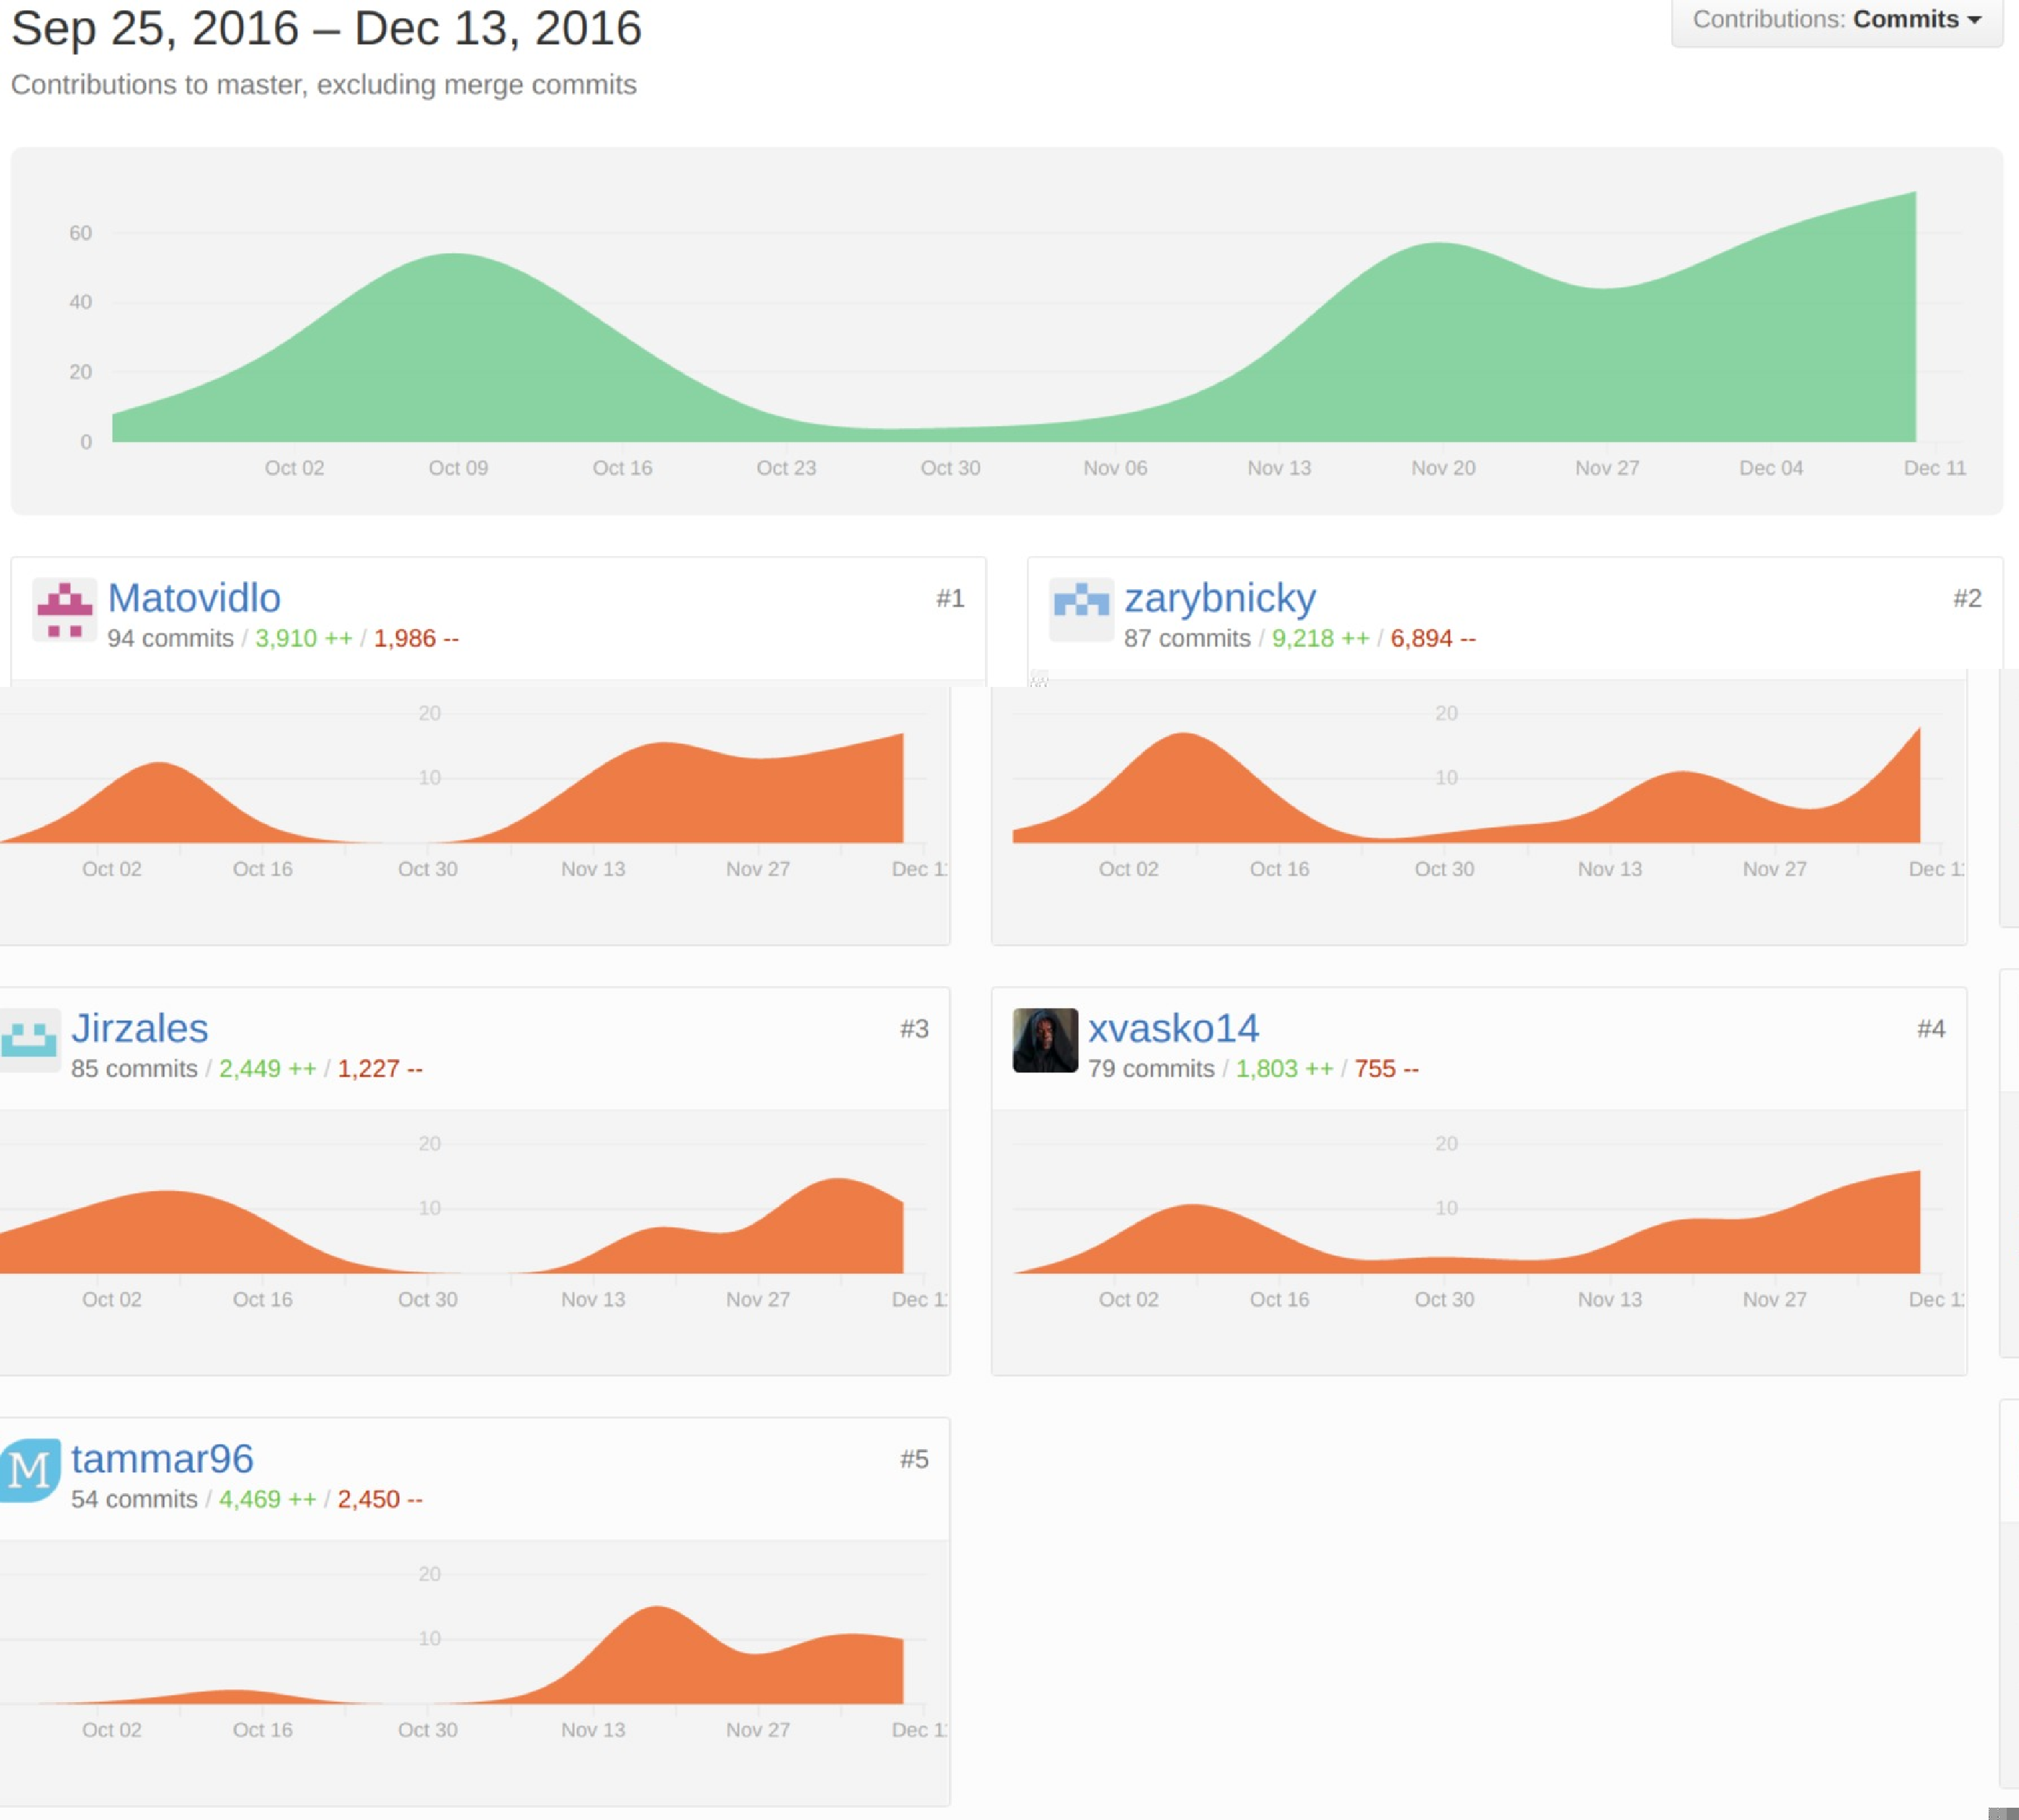
\includegraphics[width=0.65\textwidth]{./img/git_commit.pdf}
  \end{center}
\end{frame}

\begin{frame}{Počet přidaných řádků}
  \begin{center}
    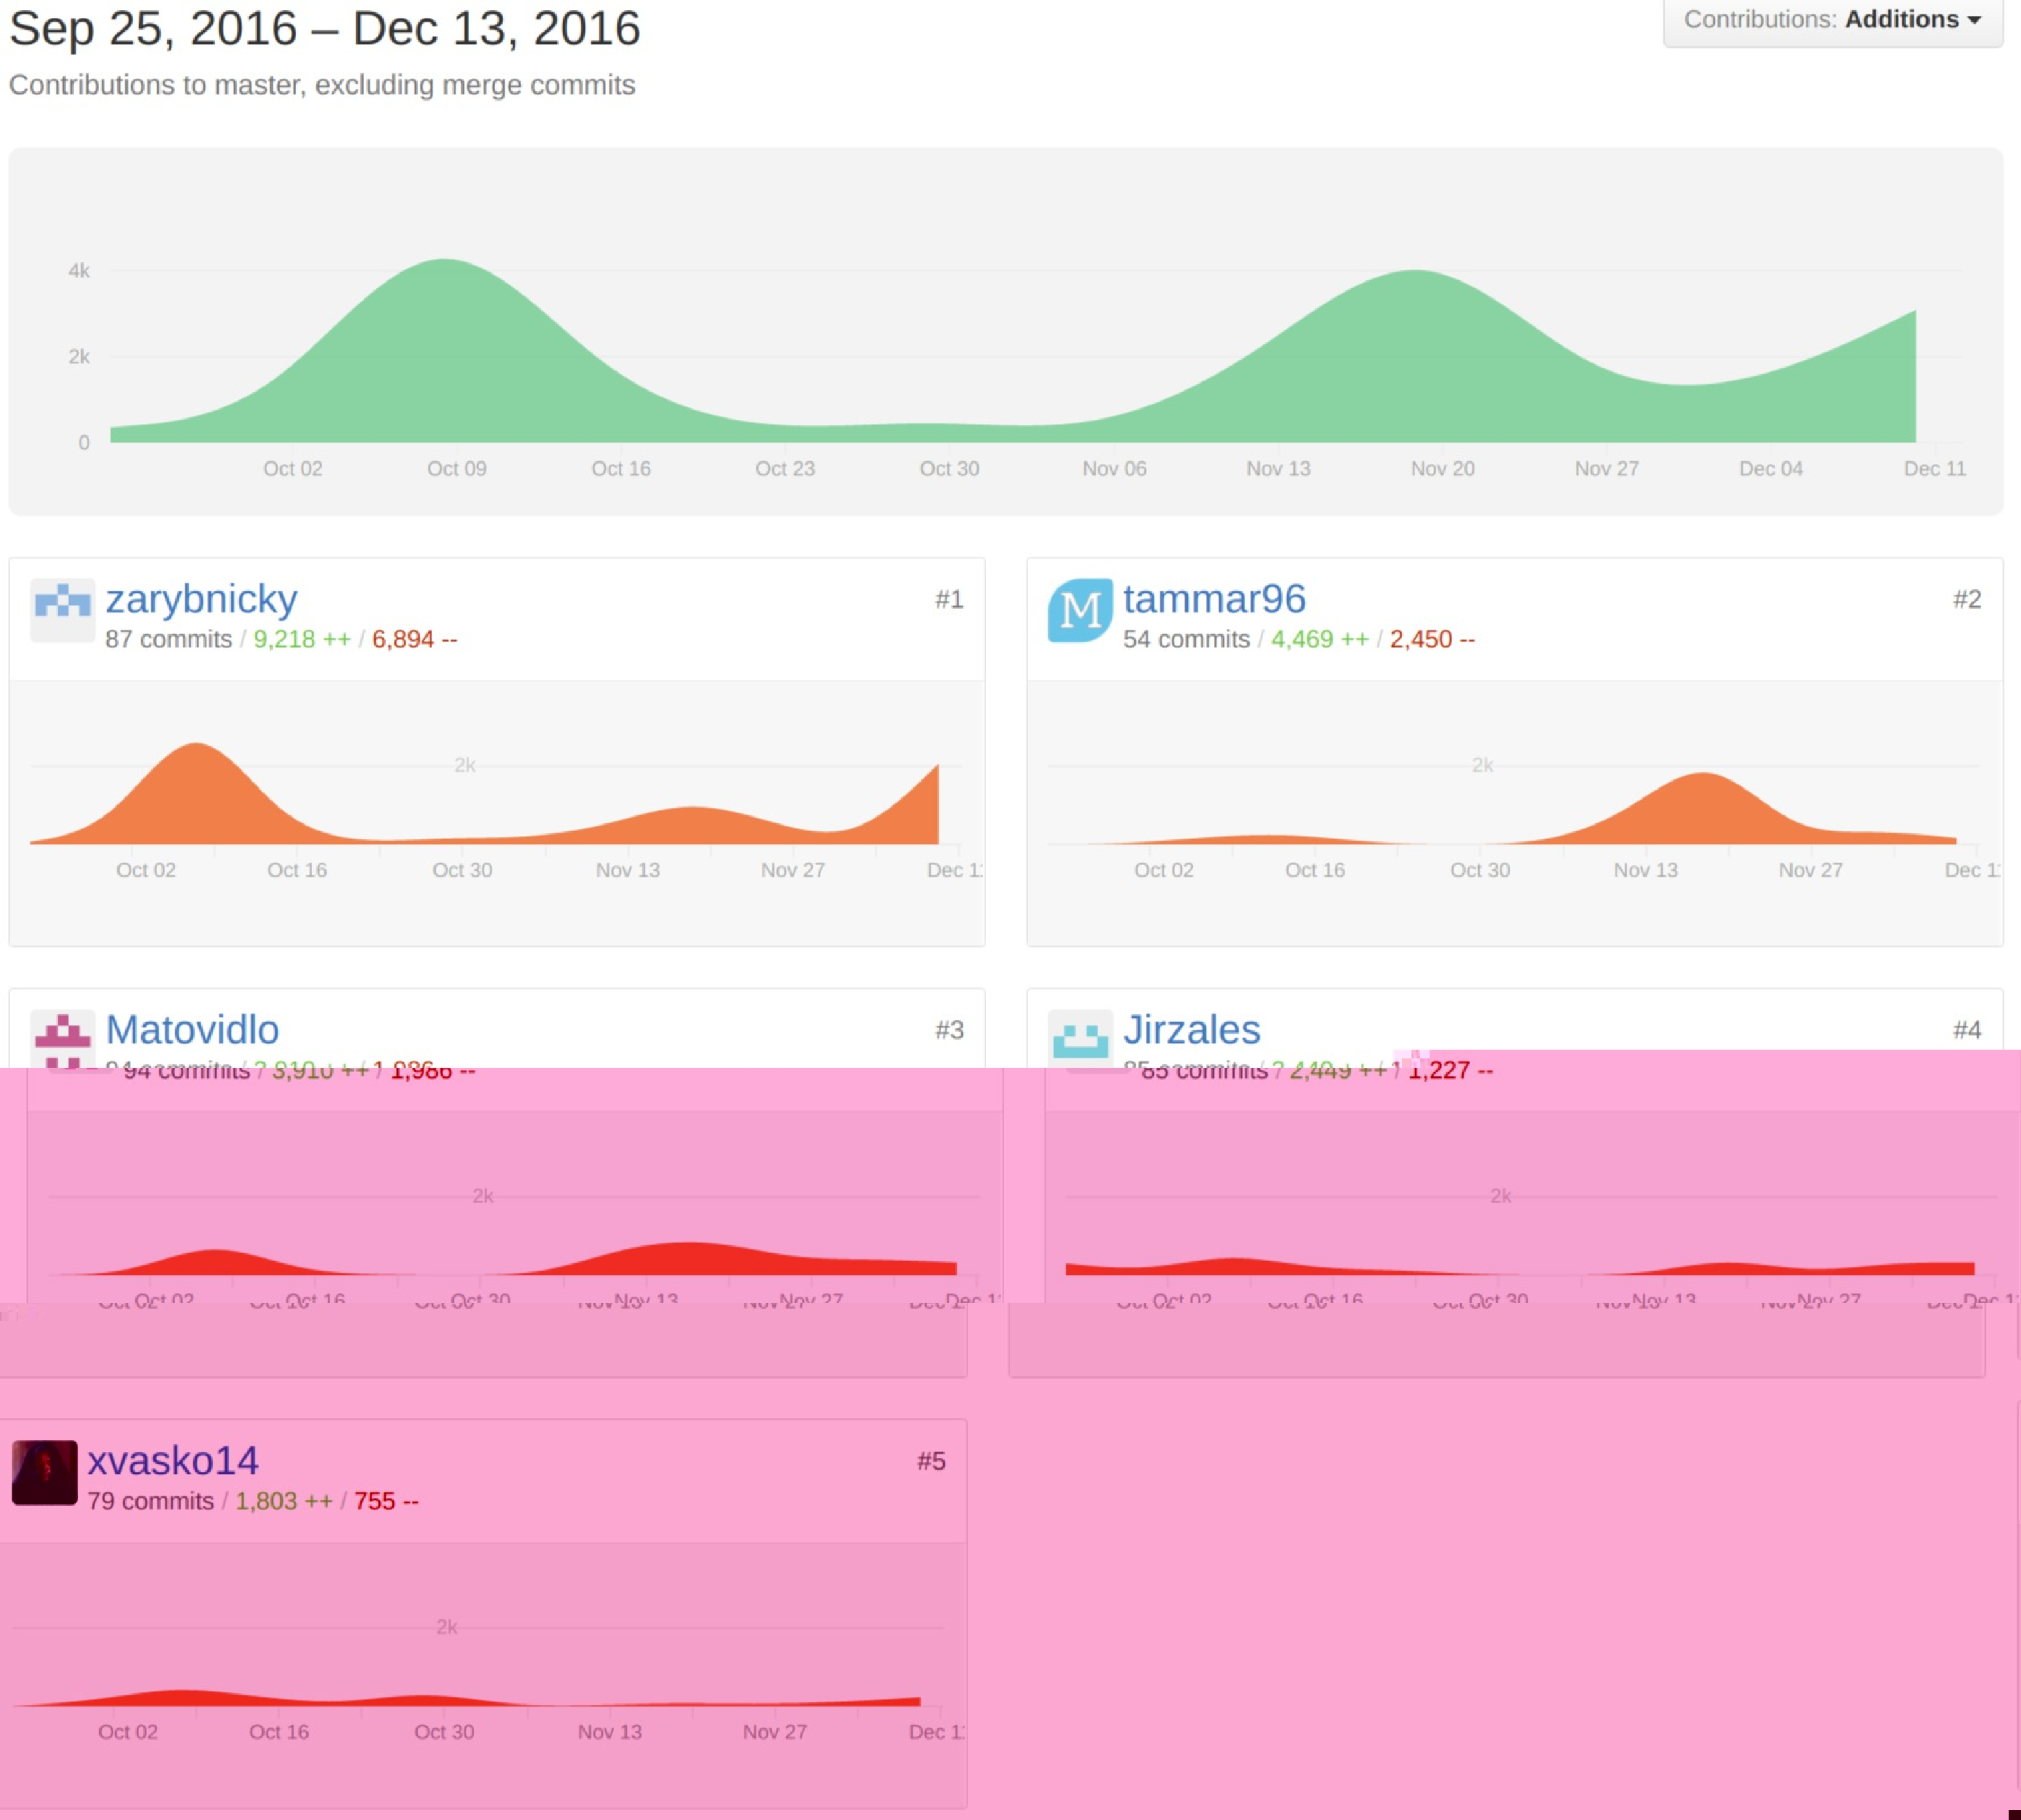
\includegraphics[width=0.65\textwidth]{./img/git_additions.pdf}
  \end{center}
\end{frame}

\begin{frame}{Počet smazaných řádků}
  \begin{center}
    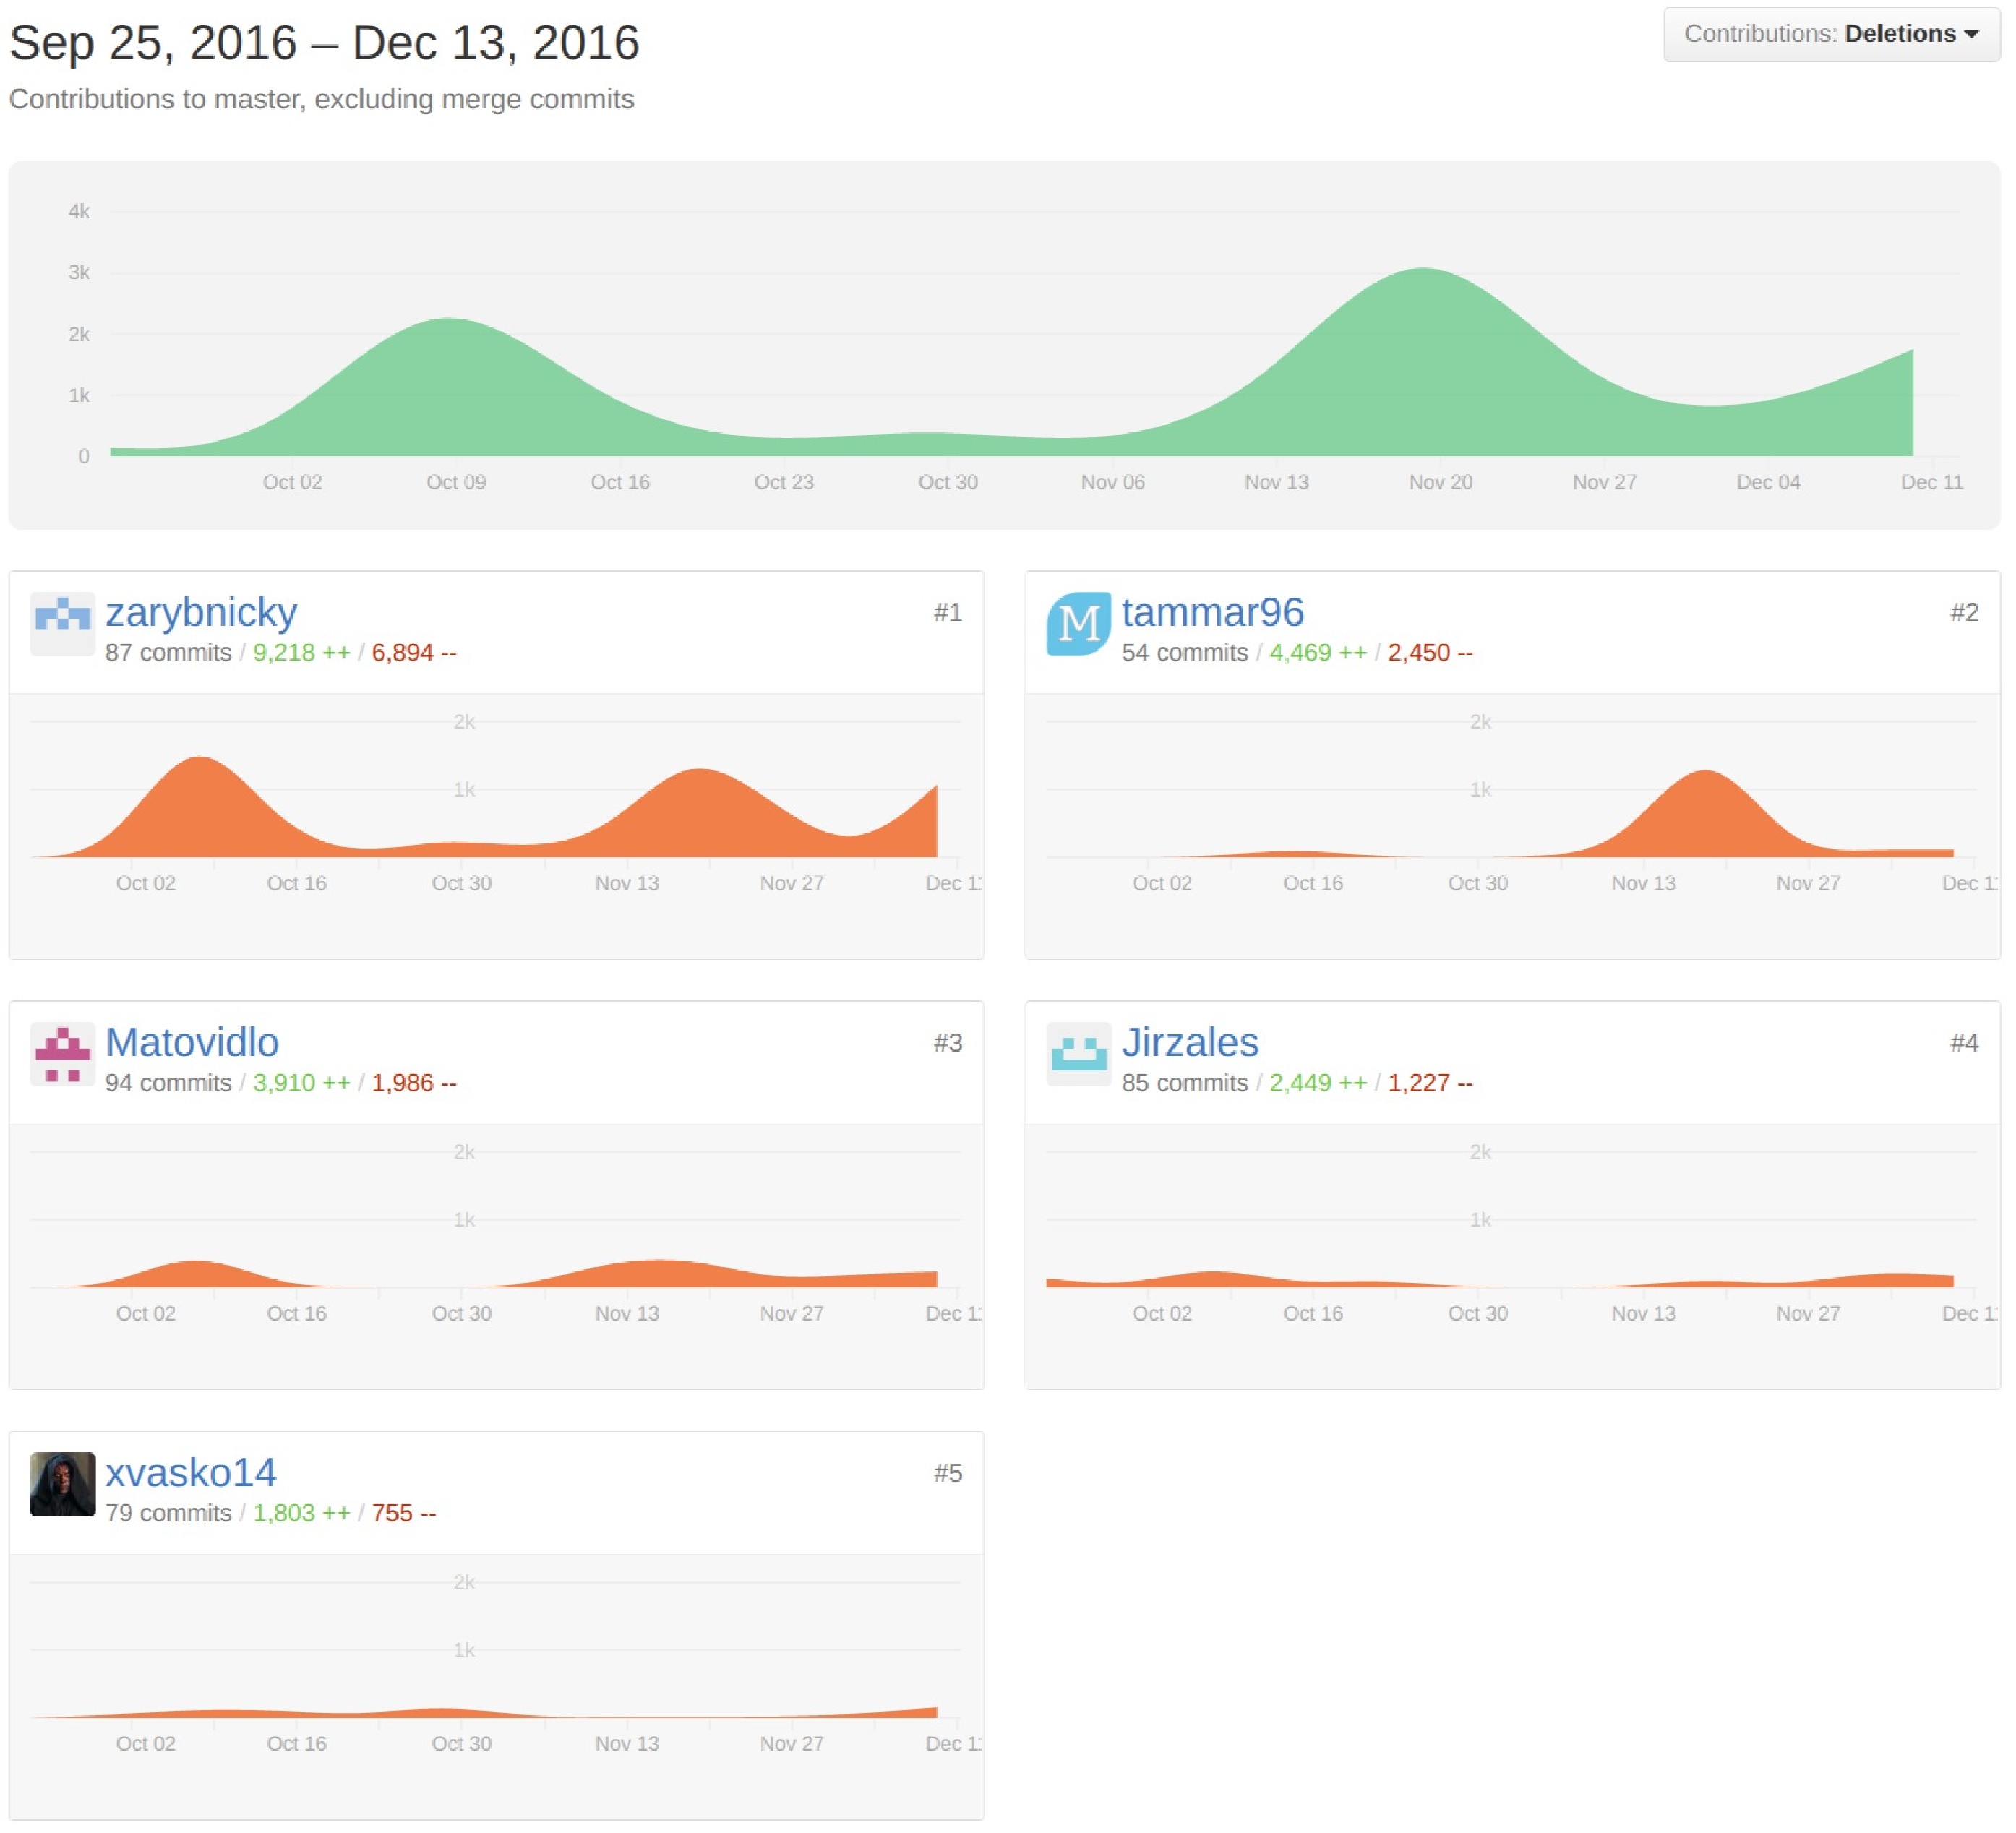
\includegraphics[width=0.65\textwidth]{./img/git_del.pdf}
  \end{center}
\end{frame}

\begin{frame}{Travis}
  \begin{center}
    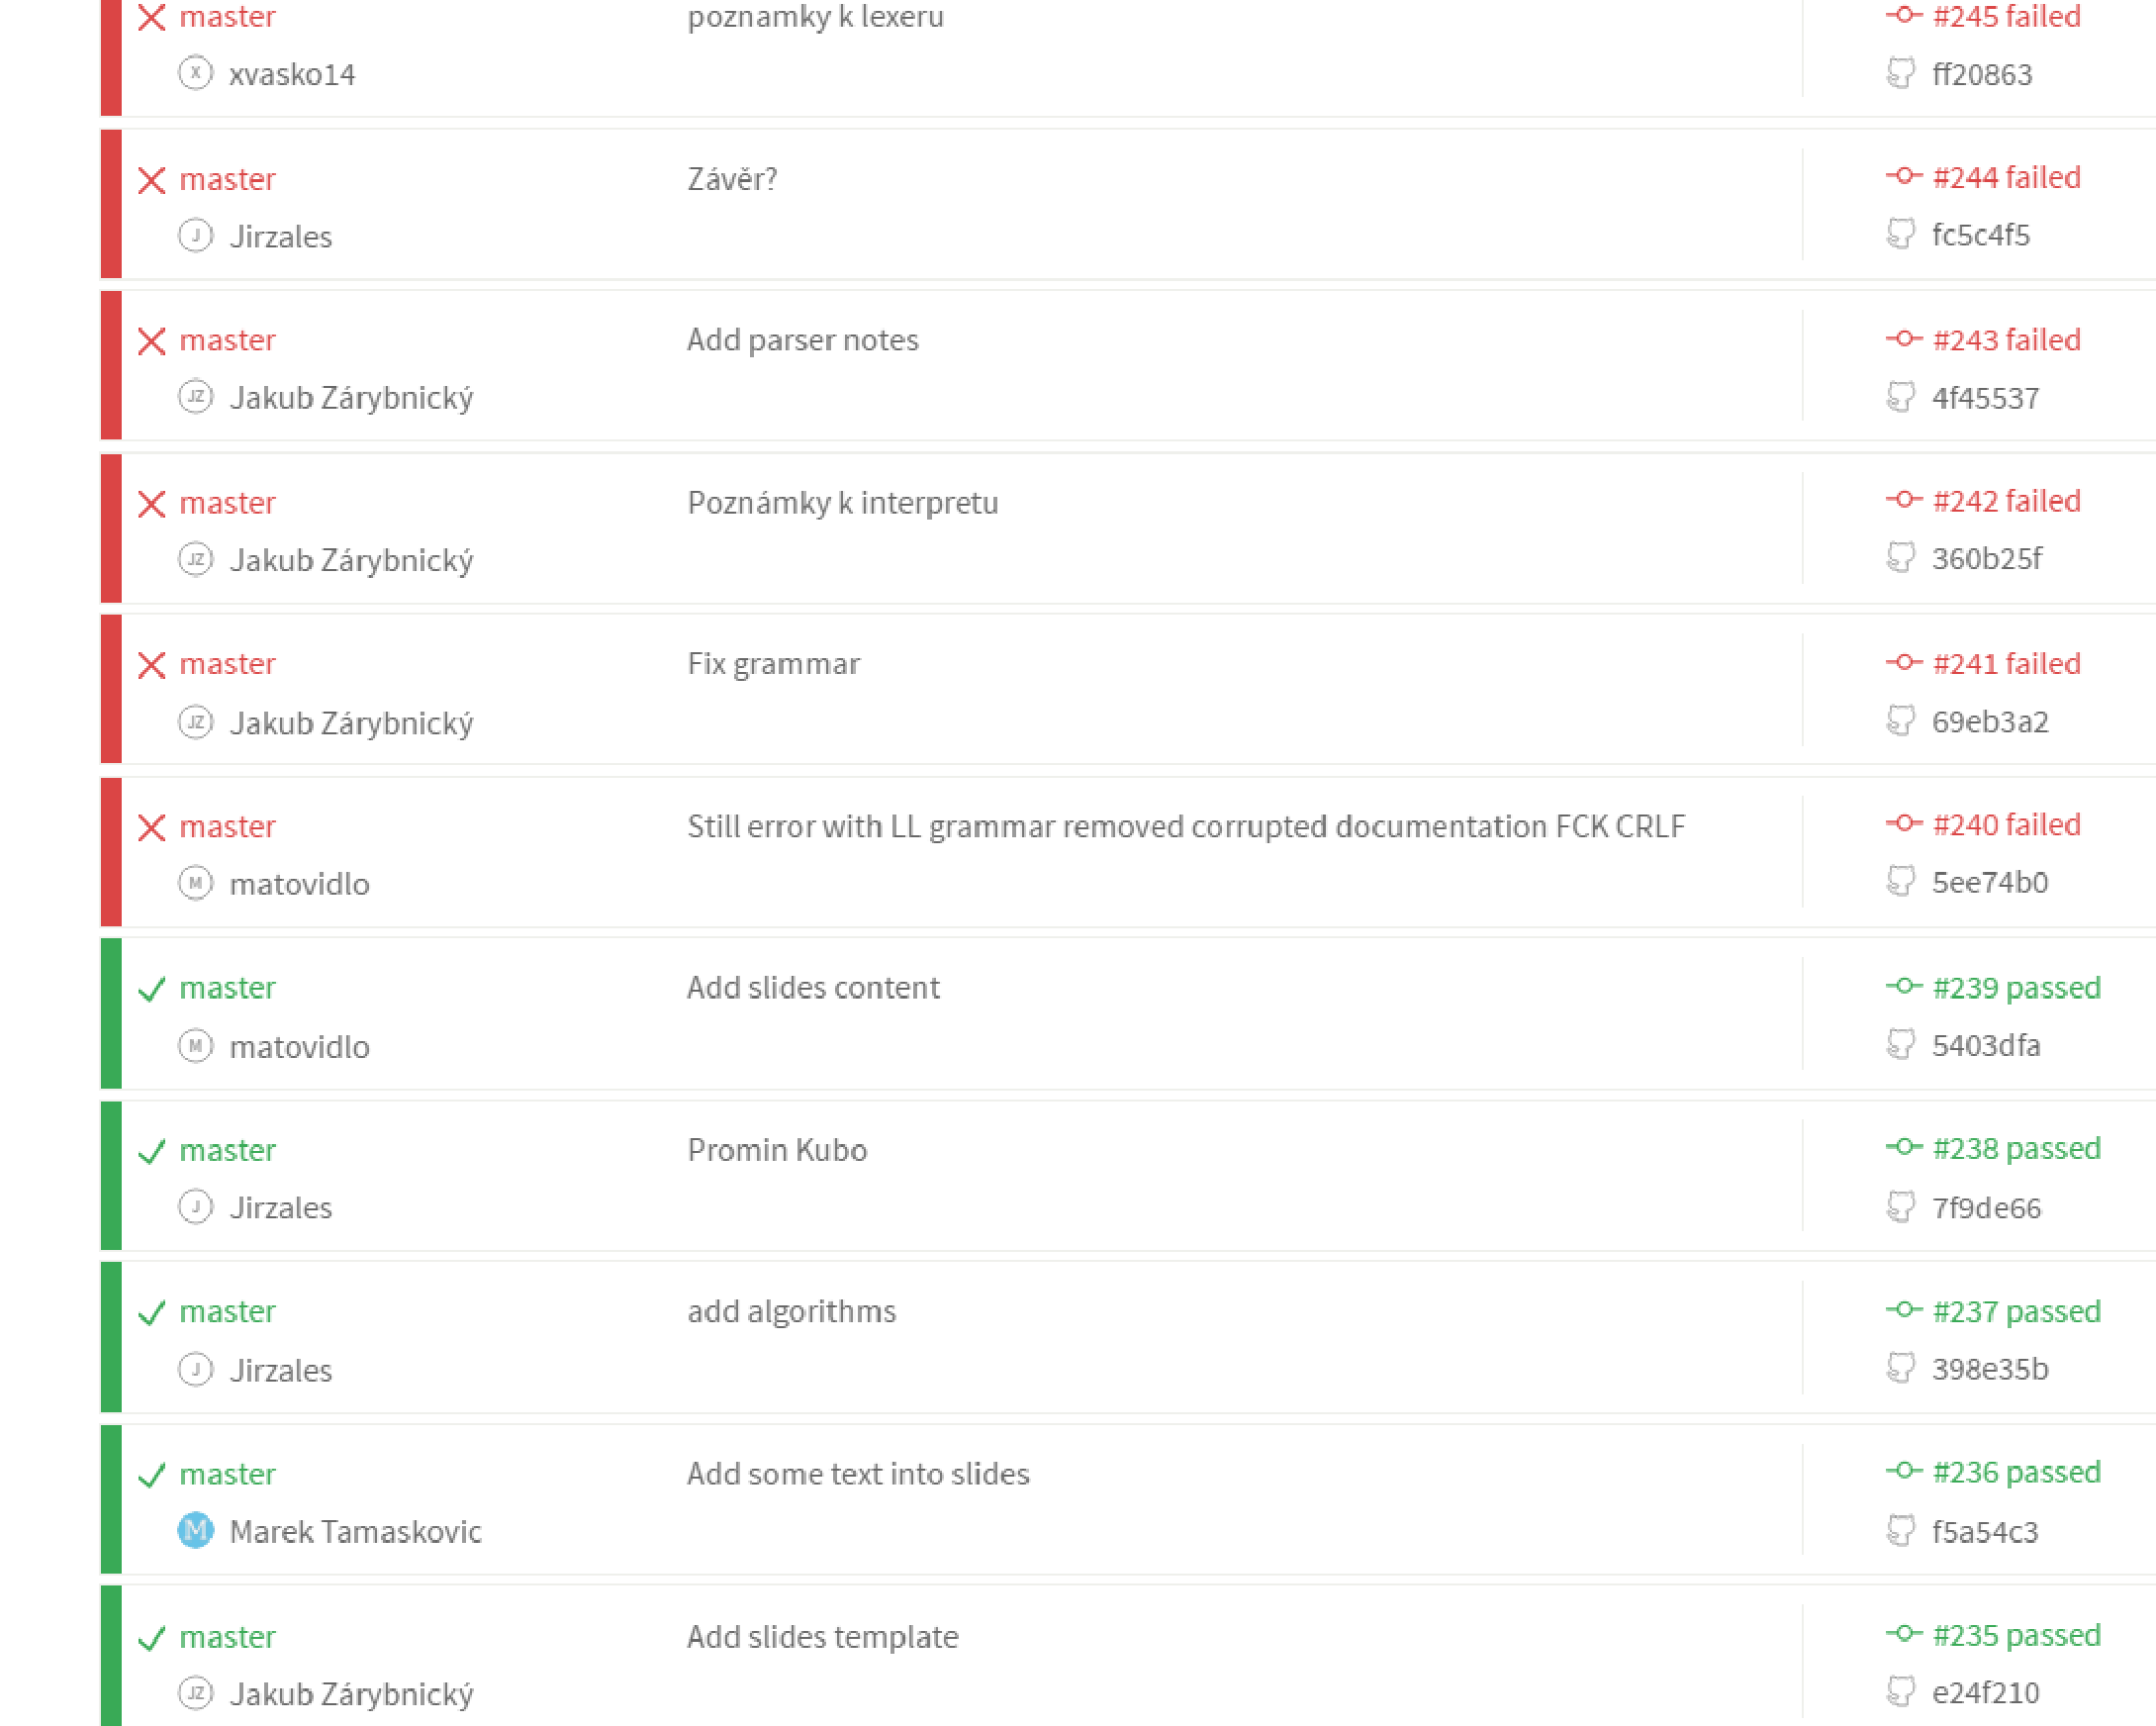
\includegraphics[width=0.65\textwidth]{./img/travis.pdf}
  \end{center}
\end{frame}

\begin{frame}{Statistiky, očekávání, rozpočet a zhodnocení}
\begin{itemize}
\item Počet souborů: \textbf{97} (\textbf{27} v C)
\item Řádky zdrojového kódu: \textbf{6622} (\textbf{5272} v C)
\item Commity v Gitu: \textbf{396}
\end{itemize}

\begin{itemize}
\item Plánované datum dokončení - 31.10.
\item Skutečné datum dokončení - 11.12.
\item Plánovaný peněžní zisk - 0 CZK/EUR
\item Finanční stav po ukončení projektu - záporný
\note[item] A dnes večer bude po teambuildingu ještě zápornější...
\end{itemize}

\end{frame}

\end{document}
